\documentclass[conference]{IEEEtran}
\usepackage{verbatim}
\usepackage{multirow} 
\usepackage[table]{xcolor}
\usepackage{enumitem}
\usepackage[normalem]{ulem}
\usepackage{graphicx} 
\usepackage{epstopdf}
\usepackage{latexsym}
\usepackage{amssymb}

\usepackage{url}
\usepackage{array}

\overfullrule 1cm

\begin{document}

\title{Change Impact Analysis Practice Under Tight Deadlines: A Case Study}

\maketitle

\begin{abstract}
  What do practitioners do when a company starts to cut corners? An
  ethnographic approach was used to observe the change impact analysis
  practice in a Malaysian company for 13 months and was followed by a
  questionnaire. First, the requirement gathering, coding, and
  in-house testing processes of the company were observed. Then, a
  questionnaire was sent to 48 software practitioners of the compnay
  with different roles across a system development life-cycle. A total
  of 27 out of 48 practitioners responded. Results showed that a
  majority of the respondents believe in quantifying and disseminating
  change impact information with other project team members. Based on
  the observation, an experiential method was used primarily for the
  project, even though the traceability-based change impact analysis
  method was required. The time limitation was a factor in this
%% Siti: required by whom? required by what?
  decision. This study employs Impact Analysis Key Questions as a
  template to summarise an impact analysis case study.
\end{abstract}


%\keywords{impact analysis, case study, practice, industry, practitioner, perception, change request, requirement, traceability}


\section{Introduction}

A change in an artifact while a system is under development and
undergoing system testing can affect the currently working software
artifacts of other practitioners. One practitioner may want and need
to know if his or her decision may affect another practitioner. For
example, a system analyst or a requirement engineer may need to ask
the software engineers to what degree changing a project's implemented
requirements can be traced to the implemented source
code. Alternately, a software engineer may need to determine from the
system analysts to what extent source code can be impacted by this
same change by tracing back to the validated requirements.

Research on requirement traceability-based change impact analysis has
emerged~\cite{ibrahim2005requirements} but it lacks empirical
analysis. Questions like the following remain: ``Will the impact
analysis method work under certain circumstances such as tight
deadlines, lack of tools, or limited resources?'' ``If method X does
not work, then will method Y work?'' It may be possible that either
some theories may not be practical or the practitioners' assumptions
may be invalid. Thus, the objective of this study was to
\textit{investigate issues pertaining to the change impact analysis
  practice of a large and complex system development project by
  observing practitioners and analysing their perceptions}.

Research collaboration with a software company's management is usually
relatively difficult.  In particular, such difficulties are faced by
software engineering researchers when studying practices in companies
that are usually not exposed to research. The faced challenges are
getting detailed information from the management about project
spending, planning, development, implementation, and testing. A
workaround solution is to work for a company and this solution has
been used for this study. Consequently, the study can be regarded as
using an \emph{ethnographic
  approach}~\cite{viller2000ethnographically}. An ethnographic
approach is a participant observation method, in which a researcher
becomes socially and physically immersed in a case to accumulate local
knowledge by mixed methods research that includes dialogues, field
notes, and/or surveys.

The presented case study is beneficial to research and practitioner
communities, as it provides a proven practical approach of change
impact analysis of a similar context. For future researchers,
%% Siti: what do you mean with "of a similar context"?
this study can provide baseline information on the current state of
categorization of change impact analysis case studies.

We present the following contributions:

\begin{enumerate}
\item A template of five key questions (\textit{what, how, who, why},
  and \textit{when}) to allow researchers to briefly present the
  essential information of empirical case studies for impact analysis.
\item A case study of a change impact analysis practice in a large and
  complex system development project.
\item A set of lessons learned, derived from the case study and the
  questionnaire.
\end{enumerate}

In the following sections, we first present related work, then we
discuss the context of the case study, followed by research questions
and results. The paper also discusses threats to validity and presents
conclusions.

\section{Related Work}

Change impact analysis has been defined by Bohner and
Arnold~\cite{arnold1993impact} as ``identifying the potential
consequences of a change, or estimating what needs to be modified to
accomplish a change''. In the following, we will discuss related work
on change impact analysis studies and on requirement-to-code analysis.

\subsection{Change Impact Analysis Studies}

Change impact analysis (CIA) topics have researched for the past 30
years. We categorize CIA studies using five key questions: what, how,
when, who and why as in Table~\ref{table:keyquestions}. The first two
key questions (\emph{what} and \emph{how}) are found in the existing
studies, and we propose to add three other key questions (\emph{who},
\emph{why} and \emph{when}). The purpose of this table is to provide a
foundation for explaining CIA case studies.

\begin{table}
\centering
\caption{Key Questions for CIA Case Studies}
\label{table:keyquestions}
\begin{tabular}{ | l @{} p{3.5cm} | p{3.5cm}|  } 
\hline
\rowcolor{lightgray} \textbf{Key}  & \textbf{Full Question} & \textbf{Examples}\\ 
\hline
What & is the software artifact type being investigated? 
\newline (The impact set, scope of artifacts) & Business Processes~\cite{mehboob2013approach} 
\newline Business Rules~\cite{oliveira2010change} 
\newline Goals~\cite{teka2012change} 
\newline Requirement~\cite{li2008requirement, nurmuliani2006requirements, davis1990software} 
\newline Architecture~\cite{tang2007using, mehboob2009approach} 
\newline UML Model~\cite{muller2014model} 
\newline Database schema~\cite{maule2008impact} 
\newline Test Cases~\cite{jainae2014tool, evans2007differential}  
\newline System Configurations~\cite{qu2011impact}  
\newline Source Code~\cite{li2013survey} 
\\ 

\hline
How & did a person investigate the software artifact change? 
\newline (The approach or method) 
& Dependency   [18-21]
\newline Traceability [6,23-25]
% Siti: link 18-21 and 6,23-25 correctly
\newline Experiential~\cite{kilpinen2008emergence} 
\newline Comparative~\cite{evans2007differential} 
\newline Historical  
\newline Manual~\cite{wetzlmaier2015improving, kilpinen2008emergence} 
\newline Automatic~\cite{von2003quatrace,briand2002automating} 
\newline Semi-Automatic~\cite{barros1995supporting} 
\\ 

\hline
Who & is involved in the software artifact change? Who needs to know the change impact?
\newline (The role) & Client Personnel 
\newline Project Manager 
\newline Requirement Engineer 
\newline System Analyst 
\newline DBA 
\newline QA Engineer 
\newline Software Tester 
\newline Software Engineer 
\newline Support Engineer 
\newline Computer 
\\

\hline
Why & is the approach used in the case study 
\newline (The reason) & Time Constraints 
\newline Presumed Experience 
\newline Tool Availability
\\

\hline
When~ & was the change impact analysis being conducted 
\newline (i.e.~The SDLC phase) & Planning 
\newline Requirement 
\newline Design 
\newline Construction 
\newline Testing 
\newline Implementation 
\newline Maintenance
\\
\hline
\end{tabular}
\end{table}


First, "\textit{what}" explains one or more types of software
artifacts being investigated or simply ``the impact sets''. The type
of impact set includes the starting, estimated and actual impact
sets such as requirement and source code.

Second, ``\textit{how}'' discusses the approaches used to analyse the
software artifact for a proposed change or simply ``the
approach''. For instance, an approach can be dependency-,
traceability-, experiential-, differential-, comparative-, or
historical-based.

The process of change impact analysis can
be either manual~\cite{wetzlmaier2015improving},
automatic~\cite{von2003quatrace,briand2002automating} and
semi-automatic~\cite{barros1995supporting}. There are several
techniques for dependency-based approaches. The dependency-based
approach impact sets can be established by examining the program
structure. The dependency techniques include
slicing~\cite{acharya2011practical}, cross-cutting
concerns~\cite{zhang2009impact}, call
graphs~\cite{badri2005supporting} and program behaviours using
symbolic execution~\cite{rungta2012change}. Traceability-based
approaches look at the mapping or linking between software
artifacts. Traceability techniques include information
retrieval~\cite{eaddy2008cerberus},
metamodel~\cite{galvao2007survey,goknil2014change}, execution
traces~\cite{ibrahim2005requirements}, and relational
database~\cite{omar2013software}.

In addition, the experiential approach uses judgment by an experienced
practitioner or the subject matter expert. For example, the
consequences of a change is decided by a technical lead of the project
team. Other ways include participating informal project team
discussions, attending formal meetings~\cite{raschke2014supporting}
and asking engineering individuals~\cite{endres2003handbook} for the
consequences of a proposed change. However, Lindvall and Sandahl’s
observed~\cite{lindvall1996practical} that ``software engineers tend
to perform impact analysis intuitively. Despite this common practice,
many software engineers do not predict the complete change impact.''

The historical approach examines at the current version of software
artifacts, studies the changes and predict the impact. The application
of this approach is by mining repositories~\cite{zimmermann2005mining,
  ying2004predicting} or singular value
decomposition~\cite{sherriff2008empirical}.

Third, the \textit{``who''} is an entity, which includes project
stakeholders or a computer program that supports the impact analysis
process. The project stakeholders include client personnel, project
managers, requirement engineers, system analysts, database
administrators, quality assurance engineers, software testers,
software engineers, and support engineers. Ali et
al.~\cite{ali2013assessing} also stressed on the importance of roles
or actors in change impact analysis projects.

Fourth, \textit{``why''} explains the reason why the specific impact
analysis approach has been chosen. Reasons for the usage of an
approach include but are not limited to, time constraints, presumed
experience, and tool availability.

Last, \textit{``when''} states in which phase of the software
development life cycle or project the impact analysis observation was
done. The project stages contain, but are not limited to, planning,
requirement, design, construction or coding, testing, implementation,
and maintenance.

\subsection{Requirement-to-code Change Impact Analysis}


There are few studies on automatically map requirement or features to
source code (requirement-to-code). Ibrahim et
al.~\cite{ibrahim2005requirements} introduced traceability technique
to support change impact analysis between requirements, system test
cases and object oriented source code. However, the technique requires
a substantial amount of manual effort 
to link requirements to others artifacts. 

Eaddy et al.~~\cite{eaddy2008cerberus} combines techniques using
information retrieval, dynamic analysis, and program analysis
techniques for locating concerns. However, they did not study impacts
of a requirement change. Egyed et al.~\cite{egyed2010effort} and Ghabi
et al.~\cite{ghabi2012code} combined techniques for validating
requirement-to-code traces but also did not study change
impact. Lehnert~\cite{lehnert2011taxonomy} states that more attention
should be paid on linking requirements, architecture, and code to
enable comprehensive impact analysis.

Zhou et al.~\cite{zhou2014collaborative} examines a collaborative
change impact analysis and mentioned that due to the variety and
complexity of dependencies, determining real impacts is hard and
usually needs interventions of a subject matter expert. Nevertheless,
Zhou et al.~have have not discusses the specific project roles of the
collaborators.

\begin{comment}
% Siti: maybe reuse parts of the following section in the related work

\section{Key Questions for Impact Analysis Studies}

In this section, we briefly present a new classification for impact
analysis case studies using five key questions. The template of the
five key questions is shown in Table~\ref{table:keyquestions}.
 
First, ``\textit{what}'' explains one or more types of software
artifacts being investigated or simply ``the impact sets''. The type
of impact set includes the starting, estimated and actual impact sets
such as requirement and source code.

Second, \textit{``how''} discusses the approaches used to analyse the
software artifact for a proposed change or simply ``the
approach''. For instance, an approach can be dependency-,
traceability-, experiential-, differential-, comparative-, or
historical-based.

Third, the \textit{``who''} is an entity, which includes project
stakeholders or a computer program that supports the impact analysis
process. The project stakeholders include client personnel, project
managers, requirement engineers, system analysts, database
administrators, quality assurance engineers, software testers,
software engineers, and support engineers.

Fourth, \textit{``why''} explains the reason why the specific impact
analysis approach has been chosen. Reasons for the usage of an
approach include but are not limited to, time constraints, presumed
experience, and tool availability.

Last, \textit{``when''} states in which phase of the Software
Development Life Cycle or project the impact analysis observation was
done. The project stages contain, but are not limited to, planning,
requirement, design, construction or coding, testing, implementation,
and maintenance.

In conclusion, the above five key questions can be used to describe
any change impact analysis case study and we utilize the key questions
in this paper to present the essential information of our study.

While there are many (impact analysis) theories, impact analysis
methods must be tested under extreme project schedules.

\begin{table*}[t]
\centering
\caption{Five Key Questions for Impact Analysis Case Studies}
\label{table:keyquestions}
\begin{tabular}{ | l | p{7cm} | p{9cm}|  } 
  \hline
  \textbf{Quest.} & \textbf{Full Questions} 
  & \textbf{Examples}\\ 
  \hline
  What & What is the software artifact type being investigated? 
         \newline (The impact set, scope of artifacts) 
  & Business Processes, Goals, Requirements, Architecture, Database schema, UML, Test Cases, System Configurations, and Source Code
  \\ 
  \hline
  How & How did a person investigate the software artifact change? 
        \newline (The approach or method) 
  & Traceability, Dependency, Experiential, Comparative, Differential, and Historical
  \\ 
  \hline
  Who & Who is involved in the software artifact change? Who needs to know the change impact?
        \newline (The role) 
  & Client, Project Manager, Requirement Engineer, System Analyst, QA Engineer, Software Engineer, Support Engineer, and Computer
  \\
  \hline
  Why & Why is the approach used in the case study? 
        \newline (The reason) 
  & Time Constraints, Presumed Experience, and Tool Availability
  \\
  \hline
  When & When was the change impact analysis being conducted? 
         \newline (i.e. The SDLC phase)
  & Planning, Requirement, Design, Construction, Testing, Implementation, and Maintenance
  \\
  \hline
\end{tabular}
\end{table*}
\end{comment}

\section{Study Context}

% Siti: Please give an introduction to the section here

The aim of the web development project was to replace a legacy system
with an enhanced system. The project was originally planned to last 8
months, and later was extended to 20 months, starting from late July
2013 and ending in early April 2015. The development effort is a
consortium of five IT companies under the management of the largest
company amongst them; the total team contains 49 staff members. The
lead company (or ``the vendor"), which is a certified
CMMI~\cite{ProductCMMIfor2010} Level 3 company, is a subsidiary of a
large IT company with approximately 1000 employees. The client is a
financial institution with a workforce of 600 employees. Both are
publicly listed companies and are located in Malaysia. For
confidentiality reasons, we cannot discuss the specifics of the
vendor's and the client's profiles and the exact deliverable
dates. The old management information system was on an IBM Lotus Notes
platform that was developed in 1998, and the system was to be replaced
with a Red Hat Linux J2EE Enterprise platform. While maintaining the
existing business functions, the new system must migrate 14 years of
data into the new system. In addition, the vendor was the same company
that had built and deployed the legacy system. The new system must be
able to manage information privacy and security issues. The
information on the client company's activities must be encrypted in
the database at certain stages because of the confidential nature of
the information. Information submission and delivery for processing
must be seamlessly integrated with some related
systems. Table~\ref{casestudycontext} depicts a summary of the case
study context.

\begin{table}
\centering
\caption{Case Study Summary}
\label{casestudycontext}
\begin{tabular}{l p{5cm}} 
\hline
Case Name & MYB 
\\
Client's Industry & Financial Institution, Malaysia.
\\
Critical Issue(s) & Performance, Privacy, and Security.
\\
Additional Information & Client may need to attend court of law session to testify and verify the information received, saved and sent out of the server. 
\\
Server & Linux (RHEL)
\\
Web Server & IBM Websphere
\\
Database & Oracle
\\
Language & Java, JSP, Javascript, HTML, CSS
\\
SDLC Type & Incremental Development
\\
Duration & From 8 months extended to 20 months
\\
Software Practitioners & 48 people + 1 author 
\\
Project Status & Successfully delivered, but over-budget
\\
\hline
\end{tabular}
\end{table}


The project had several deliverables. A contract for the project was
signed in the last week of July 2013 and was followed by a requirement
study. The requirement study was done by a group of eight
practitioners including a project manager, team lead, and six system
analysts. They were given a soft copy of a Request for Proposal (RFP)
document and given access to an existing system to be replaced, as
preliminary information to digest on the system. Later, they went to
the client site and elicited new and existing requirements against the
RFP document through formal meetings with the client's
management. Meetings were scheduled to scrutinize and validate the
requirements. To meet the critical situation of the deliverable
deadlines, many of the meetings with the client's management ended
late at night. Nevertheless, the vendor managed to get a user
requirement solutions and specifications (URSS) signed in the first
week of September 2013. Immediately after these tasks, the requirement
team began illustrating the URSS with screen designs and managed to
produce documents known as ``Screen Design Document" (SDD) by October
2013. Two separate SDD documents were created, one for the system
configuration requirement and the other for the business
requirement. During the SDD creation, the requirement team was
expanded from 8 to 10 people. Apparently, there was a need to amend
the SDD content, the team found the content to be, for two typical
reasons, mistakenly typed or technically challenging. So their
management team negotiated with the client for another sign-off that
was on 12th November 2013. The amended SDD (SDD2) was regarded as the
document baseline for the systems development.

% Siti: The table below is not referenced.
\begin{table*}[t]
\centering
\caption{Change Request Form: Impact Analysis Section}
\label{table:partb}
\begin{tabular}{|l|l|l|l|l|l|l|}
\hline
  \multicolumn{7}{|l|}{\textbf{Part - B: Impact Analysis (to be
  completed by the assigned project member \newline  )}}\\
  \hline
  \multicolumn{4}{|l|}{\begin{tabular}[c]{@{}l@{}}Impact analysis details: Reference of Requirement \\
                         Traceability Matrix (RTM)\end{tabular}} 
& \multirow{2}{*}{\begin{tabular}[c]{@{}l@{}}Estimated effort \\ for
                    change \\ (man-days)\end{tabular}} & \multirow{2}{*}{\begin{tabular}[c]{@{}l@{}}Work product\\ version to be\\ changed\end{tabular}} & \multirow{2}{*}{\begin{tabular}[c]{@{}l@{}}Verification to\\ be done \\ (tests, reviews)\end{tabular}} \\ \cline{1-4}
  & \begin{tabular}[c]{@{}l@{}}Functions / \\ features affected\end{tabular} & \begin{tabular}[c]{@{}l@{}}Work products \\ (programs, tables, \\ documents, etc)\end{tabular} & \begin{tabular}[c]{@{}l@{}}Change required \\ (description)\end{tabular} &  & &
\\ \hline 1 & \multicolumn{1}{c|}{ \ } & \multicolumn{1}{c|}{ \ } & \multicolumn{1}{c|}{ \ } & \multicolumn{1}{c|}{ \ } & \multicolumn{1}{c|}{ \ } & \multicolumn{1}{c|}{ \ }                                                                                 
\\ \hline 2 &  &  &  &  &  & 
\\ \hline
\end{tabular}
\end{table*}


While the requirement team were getting agreement on the amended
documents, the programming team had to begin their study and design on
the first version of SDD because it would be too late to wait for the
sign off on the amended document. A third team, the data migration
team, also started work early. This was because of the huge amount of
work involved to convert, clean up, and migrate the historical data
and to make the last seven years of data retrievable online. After
about ten months of development, the user acceptance testing (UAT) of
several modules was undertaken by another company outsourced by the
client. The UAT activity took place at the client's site for
approximately four months. All in all, the team managed to get the UAT
completed by November 2014 and subsequently the final acceptance test
(FAT), penetration, and performance test. \textit{The new system
  successfully went live in the third week of April, 2015.} The
project time line is summarized in Figure~\ref{fig:timeline}.

\begin{figure*}
\centering
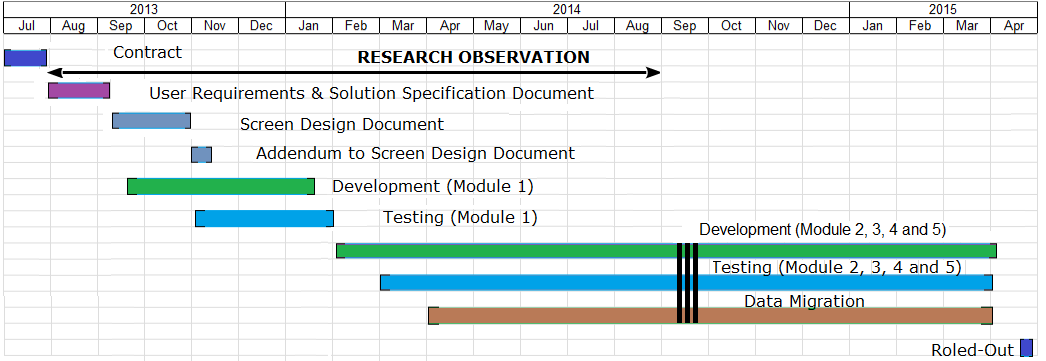
\includegraphics[width=0.9\textwidth]{pics/project422.png}
\caption{The Project Timeline: The project started in the last week of
  July 2013 and ended in early April 2015. The horizontal line depicts
  13 months of research observation. After the observation, a
  questionnaire was sent three times to the practitioners in September
  2014 as shown by the vertical stripes.}
\label{fig:timeline}
\end{figure*}

\subsection{System Description}

The six hundred pages of SDD2 business requirements describe five
large subsystems or modules: the Profile, Announcement, Internal,
Online, and Report modules. The first module (Profile Module) is an
underlying framework of all modules. It consists of user access
authentication, company profiles, session handling, and configuration
administration functions. This work-flow based framework supports
multilevel access control for different user groups for approximately
1,000 companies. The second module (Announcement Module) is a public
facing module that allows registered companies to login and publish
announcements.  The third module (Online Module) is a new function
that allows companies to register and submit applications over the
Internet to the client. During one of the requirement solicitation
meetings, a project management consultant determined that a briefly
mentioned requirement in the RFP was, in fact, a huge module by
itself. This was a scope creep and a huge setback for the already
tight deadline. Therefore, it adversely affected the project's
budget. The fourth module (Internal Application Module) supports the
day-to-day internal operational functions of the operations
department. The fifth module, the Reporting Module, extracts business
information from the other modules to facilitate management decisions.

\subsection{Change Control Processes}

The project sponsor mandated the change process and provided the
requirements team members with a change request (CR) form. The CR form
has a change impact analysis section and needed requirement
traceability matrices (RTM) as reference detailing the impacts. This
reflects the theory by Ramesh~\cite{ramesh1998factors} who established
that low-end traceability users are mandated by project sponsors. In
addition, Ali et al.~\cite{ali2013assessing} stress the importance of
detailed processes of a project's change impact analysis with roles or
actors, activities, and artifacts.

The system analysts of the requirement team (of the vendor) had to
complete the change request (CR) form, and the form had an impact
analysis section. By August 2014, the requirement team documented 56
CRs. Typical reasons for CRs were user interface design errors and
data type error found in the SDD2. The system analysts found errors in
the SDD2 documentation and informed their team lead of particular
modules. Most of the time the system analysts team lead provided an
initial approval. However, a higher authorised person (the technical
manager) had to be informed on every requirement change, regardless of
how easy the feature implementation sounded to the requirement or
coding team. For instance, a change of a requirement ranging from
``user shall press a button to display the financial year end date''
to ``user shall be able to view the financial year end date which is
automatically appeared on the screen after a web page is loaded'' is
viewed by the technical manager as a valid requirement change request
which needs the project sponsor's approval.

If a proposed change was worthy of an implementation, the technical
manager allowed the system analyst to proceed with the change
request. Then the system analysts could proceed with acquiring the
Part~B details from the project manager (PM) of the development
team. After the system analyst obtained the Part~B information, the
system analyst escalated the CR form by emailing the CR form to a
project sponsor (or client). In any case in which the Part~B
information was insufficient, the project sponsor executive returned
the CR form back to the system analyst for further clarification.

The researcher of this case study observed that the information given
for an impact was inconsistent in terms of the granularity level of
the impact sets. For instance, the CR form change impact section was
filled with classification of files (such as server, Javascript,
and/or css files). However, sometimes the CR form was filled with
medium to small granularity levels such as file names, packages,
classes, methods, and statement level.

\subsubsection{Collaboration Methods and Tool Support}

The methods of communicating requirement changes include face to face,
email, desktop chat application, office fix line and hand phone, voice
and text messages. Some of the requirement and testing team members
were stationed at the designated IT Project and UAT rooms in two
separate floors of an office building; most of the coding team members
were stationed at the IT Project Room. Neither the requirement team
nor the testing team used a RTM tool to support the project. However,
a testing consultant from a multinational IT company was present and
managed the RTM information using Microsoft Excel. The challenge was
that no dedicated tools existed for tracing artifacts. The project
team members had to use Microsoft Word and Excel to write the
requirements and to illustrate the screen designs. The team members
did not use any commercial or open source tools to accomplish the
requirement gathering, analysis, and documentation tasks.

\section{Research Questions and Results}

The ethnographical approach~\cite{viller2000ethnographically} via
observation (or case study~\cite{runeson2009guidelines}) and
survey~\cite{kasunic2005designing} was used for the data
collection. The research questions are divided by the methods of
investigation: qualitative and quantitative. RQ1 and RQ2 are two
questions for the case study; they examine the characteristics of the
impact analysis case study and the challenges of a chosen
approach. RQ3 to R8 are from the questionnaire. The unit of analysis
is an individual (a practitioner).

\subsection{Case Study Analysis}

We present two research questions for the case study.

\subsubsection{RQ1: What are the characteristics of this paper's case
  study based on the key questions?}

We use the five key questions presented in
Table~\ref{table:keyquestions} to characterize the our case study:

\begin{description}
\item[What] The software artifact type being investigated include
  requirements and source code.
\item[How] An experiential impact analysis method was used but RTM
  based traceability impact analysis approach was requested. The
  experiential method was the main method because a subject matter
  expert at the development site manually provided quick and brief
  potential change impact information based on the person's judgement.

\item[Who] At the time of the exercise of the impact analysis, the
  vendor team and client staff were involved. The vendor team includes
  roles of the technical manager, project managers, system analysts,
  DBA, testing consultant, QA engineers, functional testers, usability
  testers, software configuration manager, and software engineers. The
  client staff need the CR information and mandated use of the CR form
  in the change request processes.

\item[Why] The experiential approach was implemented because a
  decision was made by the vendor's senior management not to use a
  dedicated tool to support requirement tracing activities. A theory
  by Kitchenham et al.~\cite{kitchenham2004evidence} explains that a
  technology adoption is often decided either by project managers on a
  project by project basis or senior managers on a departmental or
  organizational basis. In addition, the project already had a tight
  schedule and needed to focus on delivering what was necessary. On
  top of that, the testing consultant who was maintaining the
  requirement traces already advised the vendor's senior management
  about a commercial dedicated tool which can be used to support the
  artifact tracing tasks. However, the vendor management did not agree
  to use the commercial tool as suggested by the testing
  consultant. The subject matter expert with presumed experience was
  providing the required impact analysis information.

\item[When] The analysis was during the construction and second
  module's user acceptance testing.
\end{description}

% Siti: Please provide some concluding remarks on the above

\subsubsection{RQ2: What are the challenges of the Impact Analysis
  approach implemented in the project?}

A few challenges are presented. First, the experiential and
traceability based impact analysis approaches result in impact sets
inconsistency of impact sets in terms of the source code granularity
level. For a project of a similar context, the experiential approach
can be used but not without caution. To implement the experiential
approach, the software development management must recognize that a
subject matter expert needs to have certain characteristics. The
person must be approachable, have outstanding memory and logical
thinking capability, be a very good communicator and be able to cope
with stress. Second, RTM based impact analysis cannot be practised
efficiently until the traceability researchers have resolved the
traceability challenges~\cite{gotel2012grand}.
% Siti: What are the challenges?
Third, at times the development team lead gave sketchy change impact
analysis information because providing source code details to the
system analysts was time consuming. Fourth, the impact was not
communicated in numerical value; thus, a tendency was to delay in
decision making as managers and team leads thought of the magnitude of
the change impact.

\subsection{Questionnaire Response Analysis}

After 13 months of observation, the author left the company and
emailed a questionnaire to the practitioners.  A statement to protect
the identity of the respondents was clearly conveyed. The
questionnaire was designed to reflect the case study by emphasising
the relevant artifact types, which were the \emph{requirements} and
the \emph{source code}.

An estimation for a practitioner to spend time answering six questions
was about 5--8 minutes. The author sent the questionnaire during the
project's second module user acceptance test. In total, we sent three
email reminders, and the result was that 27 out of 48 personnel
answered (an additional 4 respondents abandoned the questionnaire
halfway). The response rate was 56\%. 

A total of 4 out of 6 questions from the survey were analysed and
elaborated in RQ3 to RQ8. However, the 5th and 6th (last) are not
discussed and do not have valuable information and therefore are not
presented due to space limitations.

\begin{enumerate}
\item I work as an IT personnel for:
  \begin{enumerate}
  \item Less than 3 years
  \item 3 to 5 years
  \item 6 to 8 years
  \item 9 to 11 years
  \item More than 11 years
  \end{enumerate}

\item I am assigned to work at this SDLC stage(s):\\
  (Select ONE OR MORE) \\
  $\Box$~Planning\\
  $\Box$~Requirement\\
  $\Box$~Design\\
  $\Box$~Development\\
  $\Box$~Testing\\
  $\Box$~Implementation\\
  $\Box$~Maintenance
\item Please rate each statement on a Likert scale from 1 to 5\\
 (1: Strongly Disagree, 2: Disagree, 3: Neither Disagree Nor Agree, 4:
 Agree, 5: Agree)
 \begin{enumerate}
 \item A change in the requirement can have an impact on the source code. 
 \item A change in the source code can have an impact on the requirements. 
 \item Any change in one of the software artifacts can affect other artifacts.
 \item The requirements impacted by a source code change should be searchable.
 \item The requirements impacted by a source code change should be ranked according to the severity of the impact.	
 \item Information on the consequences of changing a requirement should be disseminated amongst the other members of the team.
 \item It would help team members to make informed decision if the impact can be quantified
 \end{enumerate}

\item Are you working with the source code in the recent project? (Yes/No)
\end{enumerate}

\begin{table}
\caption{Practitioners' Responses for Questions 1--5}
\label{table:response}
\scriptsize
\begin{tabular}{|c|c@{~~}|c@{~~}c@{~~}c@{~~}c@{~~}c@{~~}c@{~~}c@{~~}c|c@{~~}c@{~~}c@{~~}c@{~~}c@{~~}c@{~~}c|c|c|c|}
\hline
\rowcolor{lightgray} &  \textbf{Q1}    & \multicolumn{8}{c|}{\textbf{Q2}} & \multicolumn{7}{c|}{\textbf{Q3}} & \textbf{Q4} & \\
\rowcolor{lightgray} \textbf{P} & \textbf{E1} & \textbf{E2} & \textbf{P} & \textbf{R} & \textbf{d} & \textbf{D} & \textbf{T} & \textbf{I} & \textbf{M} & \textbf{a} & \textbf{b} & \textbf{c} & \textbf{d} & \textbf{e} & \textbf{f} & \textbf{g} & \textbf{S} & \textbf{G} \\
\hline
1 & 5 & 3 &  &  &  & \checkmark & \checkmark & \checkmark  &  & 4 & 4 & 4 & 4 & 4 & 4 & 4 & Y & M \\
\hline
2 & 5 & 3 &  &  & \checkmark & \checkmark & \checkmark &   &  & 4 & 2 & 3 & 3 & 4 & 4 & 4 & Y & M \\
\hline
3 & 5 & 2 &  &  &  & \checkmark &  & \checkmark  &  & 5 & 4 & 4 & 4 & 4 & 5 & 5 & Y & F \\
\hline
4 & 4 & 5 &  &  & \checkmark & \checkmark & \checkmark & \checkmark  & \checkmark & 5 & 3 & 5 & 5 & 5 & 5 & 5 & Y & M \\
\hline
5 & 4 & 4 & \checkmark & \checkmark &  &  & \checkmark &   & \checkmark & 4 & 4 & 4 & 4 & 4 & 4 & 4 & Y & F \\
\hline
6 & 4 & 4 &  &  &  & \checkmark & \checkmark & \checkmark  & \checkmark & 5 & 5 & 4 & 4 & 4 & 4 & 4 & Y & M \\
\hline
7 & 4 & 3 &  &  &  & \checkmark &  & \checkmark  & \checkmark & 5 & 1 & 5 & 3 & 4 & 4 & 4 & Y & M \\
\hline
8 & 4 & 3 &  &  & \checkmark & \checkmark & \checkmark &   &  & 4 & 4 & 4 & 4 & 5 & 5 & 5 & Y & M \\
\hline
9 & 3 & 3 &  &  & \checkmark & \checkmark &  &   & \checkmark & 4 & 2 & 2 & 3 & 3 & 3 & 4 & Y & M \\
\hline
10 & 3 & 3 &  &  & \checkmark & \checkmark & \checkmark &   &  & 5 & 1 & 5 & 3 & 2 & 5 & 5 & Y & F \\
\hline
11 & 3 & 1 &  &  &  & \checkmark &  &   &  & 5 & 1 & 2 & 4 & 4 & 5 & 4 & Y & M \\
\hline
12 & 2 & 7 & \checkmark & \checkmark & \checkmark & \checkmark & \checkmark & \checkmark  & \checkmark & 5 & 2 & 2 & 4 & 4 & 5 & 5 & Y & M \\
\hline
13 & 2 & 6 & \checkmark & \checkmark &  & \checkmark & \checkmark & \checkmark  & \checkmark & 4 & 4 & 3 & 4 & 4 & 4 & 4 & Y & M \\
\hline
14 & 2 & 2 &  &  &  & \checkmark &  &   & \checkmark & 5 & 5 & 5 & 5 & 5 & 5 & 5 & Y & M \\
\hline
15 & 2 & 1 &  &  &  & \checkmark &  &   &  & 4 & 2 & 4 & 4 & 4 & 4 & 4 & Y & F \\
\hline
16 & 1 & 4 &  &  & \checkmark & \checkmark & \checkmark & \checkmark  &  & 5 & 4 & 5 & 5 & 5 & 5 & 4 & Y & M \\
\hline
17 & 1 & 1 &  &  &  & \checkmark &  &   &  & 5 & 3 & 4 & 4 & 4 & 4 & 4 & Y & M \\
\hline
18 & 5 & 4 &  & \checkmark & \checkmark &  & \checkmark &   & \checkmark & 5 & 3 & 3 & 4 & 4 & 5 & 4 & N & M \\
\hline
19 & 5 & 4 & \checkmark & \checkmark & \checkmark &  & \checkmark &   &  & 4 & 4 & 4 & 3 & 4 & 4 & 4 & N & M \\
\hline
20 & 5 & 2 &  & \checkmark &  &  & \checkmark &   &  & 5 & 5 & 5 & 5 & 5 & 5 & 5 & N & F \\
\hline
21 & 5 & 1 & \checkmark &  &  &  &  &   &  & 4 & 4 & 4 & 4 & 4 & 4 & 5 & N & F \\
\hline
22 & 3 & 7 & \checkmark & \checkmark & \checkmark & \checkmark & \checkmark & \checkmark  & \checkmark & 4 & 3 & 3 & 4 & 5 & 4 & 4 & N & F \\
\hline
23 & 3 & 5 & \checkmark & \checkmark & \checkmark & \checkmark & \checkmark &   &  & 4 & 3 & 3 & 4 & 5 & 4 & 3 & N & F \\
\hline
24 & 3 & 1 &  &  &  &  & \checkmark &   &  & 5 & 5 & 4 & 5 & 5 & 5 & 4 & N & F \\
\hline
25 & 1 & 5 & \checkmark & \checkmark & \checkmark &  & \checkmark &   & \checkmark & 4 & 4 & 4 & 3 & 3 & 3 & 4 & N & F \\
\hline
26 & 1 & 4 & \checkmark & \checkmark & \checkmark &  & \checkmark &   &  & 5 & 5 & 3 & 4 & 4 & 4 & 4 & N & M \\
\hline
27 & 1 & 1 &  &  &  &  & \checkmark &   &  & 5 & 5 & 4 & 4 & 4 & 5 & 5 & N & M \\
\hline
\end{tabular}
\end{table}

% BEGIN: SURVEY QUESTIONS
% QUESTION 1

Table~\ref{statisticsquestion3} shows descriptive statistics for
survey Question~3, a) to g). We assigned labels to each of the
questions. Requirement-to-Code has a weighted average of 4.56 with a
standard deviation of 0.50 and Code-to-Requirement has a weighted
average of 3.41 and standard deviation of 1.28. Figure~\ref{histogram}
% Siti: the referenced picture is for histograms
illustrates two boxplots for a)~Requirement-to-Code and
b)~Code-to-Requirement showing difference of the weighted average or
mean.

\subsubsection{RQ3: Does a practitioner believe that changing a
  requirement can impact the source code (requirement-to-code) is
  equal to believing the reverse (code-to-requirement)?}

We would like to know if there is a difference in opinions between the
requirement-to-code and code-to-requirement. We expect that there is
no difference in perceptions for requirement-to-code and
code-to-requirement because of the \emph{bidirectional traceability}
praxis~\cite{ProductCMMIfor2010}. So it is sensible to have a null
hypothesis of ``no difference''.

\begin{enumerate}[ ] 
\item $H_o$: No difference in perceptions 
\item $H_a$: Has difference in perceptions
\end{enumerate} 

\begin{table*}
\caption{The Frequency, Weighted Average And Standard Deviation for Survey Question~3}
\label{statisticsquestion3}
\centering
\begin{tabular}{|c|l|c|c|c|c|c|c|c|}
\hline
\rowcolor{lightgray} &  Statement  &  1 & 2 & 3 & 4 & 5 & W-Avg. & Std Dev.  
\\
\hline
a & \textbf{Requirement-to-code}   & 0\% & 0\% & 0\% & 44\% & 55\% & 4.56 & 0.50 
\\
\hline
b & Code-to-requirement  & 11\% & 15\% & 19\% & 33\% & 22\% & 3.41 & 1.28
\\
\hline
c & Other artifacts       & 0\% & 11\% & 22\% & 44\% & 22\% & 3.78 & 0.92
\\
\hline
d & Searchable            & 0\% & 0\% & 22\% & 59\% & 19\% & 3.96 & 0.64
\\
\hline
e & Ranked                & 0\% & 4\% & 7\% & 63\% & 26\% & 4.11 & 0.68
\\
\hline
f & \textbf{Disseminated}          & 0\% & 0\% & 7\% & 48\% & 44\% & 4.37 & 0.62
\\
\hline
g & \textbf{Quantified Impact}             & 0\% & 0\% & 4\% & 63\% & 33\% & 4.30 & 0.53
\\
\hline
 
\end{tabular}
\end{table*}


\begin{figure}
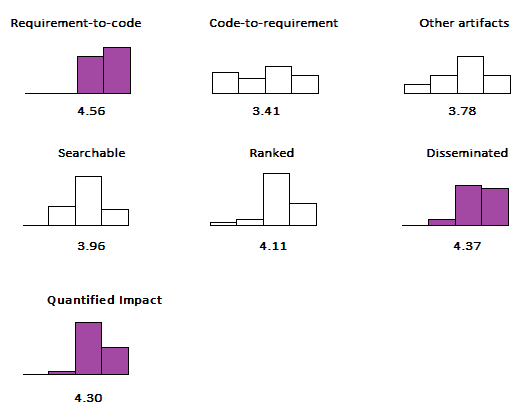
\includegraphics[width=\columnwidth]{pics/multihist.png}
\caption{Histogram: Practitioners' agreement on Question 3, a)--g)}
\label{histogram}
\end{figure}

Using 27 rows of response data tabulation in
Table~\ref{table:response}, we analysed that there is a difference in
perception for Questions 3a and 3b.  A paired t-test shows
$t(26) = 4.3278$, $p < 0.05$, and indicates that the difference is
statistically significant. The two-tailed $p$-value equals 0.0002 at
95\% confidence interval (0.05 significance level) and by conventional
criteria, this difference is considered to be statistically
significant.

$H_o$ states that there is no significant difference between
practitioners' opinions on requirement-to-code and
code-to-requirement. However, in this case, we reject $H_o$. In other
words, we do not agree with $H_o$ and choose $H_a$. Therefore, there
is a significant difference between practitioners' perceptions of
requirement-to-code and code-to-requirement change
impacts. \textbf{\textit{Surprisingly, a belief in forward
    traceability change impact is statistically significant (rather
    than the reverse or bidirectional).}}

\subsubsection{RQ4: Does a practitioner believe any change in one of
  the software artifacts can affect other artifacts?} 

Not all practitioners believe that any change in one of the software
artifacts can affect other artifacts. Table~\ref{statisticsquestion3},
Row~c shows that 11\% did not agree, 22\% neither agreed nor
disagreed, 44\% agreed, and 22\% strongly agreed. Question~3c (``Other
artifacts'') depicts a weighted average of 3.78 and standard deviation
of 0.92, meaning that the practitioners' opinions vary. \textit{The
  11\% practitioners have 3 to 8 years of experience and were involved
  in coding recently but we are unable to find a valid explanation to
  why they did not agree}. Still, a weak majority (67\%) of
practitioners agreed that change in one of the software artifacts can
affect other artifacts. This indicate that the practitioners do
believe in the importance of change impact analysis in projects.

\subsubsection{RQ5: Does a practitioner agree that requirements
  impacted by a source code change should be searchable?}

Practitioners agreed or were neutral on this
matter. Table~\ref{statisticsquestion3}, Row~d shows that 22\% neither
agreed nor disagreed, 59\% agreed and 19\% strongly
agreed. Question~3d (``Searchable'') shows a weighted average of 3.96
and standard deviation of 0.64, meaning that the practitioners'
opinions are somewhat disperse. A weak majority (78\%) of
practitioners agreed that requirements impacted by a source code
change should be searchable.

\subsubsection{RQ6: Does a practitioner agree that requirements
  impacted by a source code change should be ranked according to the
  severity of the impact?}

Not all practitioners agreed on this. Question~3e shows that 4\% did
not agree, 7\% neither agreed nor disagreed, 63\% agreed and 26\%
strongly agreed. Question~3e (``Ranked'') describes a weighted average
of 4.11 and standard deviation of 0.68, meaning that the
practitioners' opinions are not so disperse. A majority (89\%) of
practitioners agreed that requirements impacted by a source code
change should be ranked according to the severity of the impact.

\subsubsection{RQ7: Does a practitioner agree that requirements
  impacted by a source code change should be disseminated amongst the
  other members of the team?} 

Answers were either agreed or neutral. Question~3f stated that 7\%
neither agreed nor disagreed, 48\% agreed, and 44\% strongly
agreed. Table \ref{statisticsquestion3} of Question~3f
(``Disseminated'') illustrates a weighted average of 4.37 and standard
deviation of 0.62, meaning that the practitioners' opinions are
alike. A strong majority (93\%) of practitioners agreed that
requirements impacted by a source code change should be disseminated
amongst the other members of the team.\textbf{\textit{This result
    shows the importance of informing all teams across multiple SDLC
    phases on the change impacts analysis results.}}

\subsubsection{RQ8: Does a practitioner agree that it would help team
  members to make an informed decision if the impact can be
  quantified?} 

Answers were either agreed or
neutral. Table~\ref{statisticsquestion3}, Row~g stated that 7\%
neither agreed nor disagreed, 48\% agreed, and 44\% strongly
agreed. Table \ref{statisticsquestion3} of Question~3f (``Quantified
Impact'') illustrates a weighted average of 4.30 and standard
deviation of 0.53, meaning that the practitioners' opinions are
similar. Almost all (96\%) practitioners agreed. \textbf{\textit{This
    study suggests that a practitioner should convey a numerical value
    of an impact magnitude to other team members so that it would help
    team members make an informed decision.}}

\subsubsection{Trend} 

Given the responses in Table~\ref{table:response}, we looked into
patterns of three groups. The groups are those who have the
requirement role, the coding and the noncoding roles. Practitioners
who have requirement roles are distinctly identified from Q2
(Column~R), source code related roles from Question~2 and also by Q4
(Column~S).  In each analysis, we emphasise strong positive or
negative values that have correlation coefficient 0.7 and
above. Table~\ref{tab:legend} shows the meaning of the rows and
columns of the following tables for the three different roles.

\begin{table}
\centering
\caption{Meaning of the rows and columns in tables~\ref{table5},
  \ref{table6}, and \ref{table7}.}
\label{tab:legend}
\begin{tabular}{|rl|}
\hline
$E1$ & Experience in number of years  (Q1)\\
$E2$ & Experience in number of roles (Q2)\\
a. & Requirement-to-code (Q3a)\\ 
b. & Code-to-requirement (Q3b)\\
c. & Other artifacts (Q3c)\\
d. & Searchable (Q3d)\\
e. & Ranked (Q3e)\\
f. & Disseminated (Q3f)\\
g. & Quantified Impact (Q3g)\\
G. & Gender\\
\hline
\end{tabular}
\end{table}

\paragraph{Requirement Role}

Table~\ref{table5}, row $E2$ and column (b, c) has a correlation
coefficient of -0.73 and -0.78 respectively. This reveals that
experience of having a number of roles has a strong negative linear
relationship with perception b (``Code-to-requirement'') and c
(``Other artifacts''). \textbf{\textit{A person who is currently under
    a requirement team and has experience having other roles (such as
    a software engineer, software tester, DBA, or any other software
    roles) is less likely to believe that changing code can impact the
    implemented requirements or any change in an artifact will impact
    other artifacts.}}

\begin{table}[ht]
\centering
\caption{Correlation Between Experience, Question 3a-g and Gender (Requirement Role) }
\label{table5}
\begin{tabular}{|c|rrrrrrr|r|}
\hline
\rowcolor{lightgray} & a~~ & b~~ & c~~ & d~~ & e~~ & f~~ & g~~ & G~~ \\
\hline
E1 & 0.08   & 0.02 & 0.46 & 0.26 & 0.48 & 0.53 & 0.11 & 0.07  \\
\hline
E2 & -0.31   & \textbf{-0.73} & \textbf{-0.78}  & -0.28 & -0.10 & -0.18 & -0.10 & -0.14 \\
\hline
\end{tabular}
\end{table}


\paragraph{Coding Role}

Table~\ref{table6} illustrates the correlation coefficient between
number of experience (E1), experience of having number of roles (E2),
3a-g and gender (G). These factors had no significant correlations
with each other.

\begin{table}[ht]
\centering
\caption{Correlation Between Experience, Question 3a-g and Gender (Coding Role) }
\label{table6}
\begin{tabular}{|c|rrrrrrr|r|}
\hline
\rowcolor{lightgray} & a~~ & b~~ & c~~ & d~~ & e~~ & f~~ & g~~ & G~~ \\
E1 & -0.26   & 0.03 & 0.02 & -0.34 & -0.07 & -0.09 & 0.09 & 0.14 \\ 
\hline
E2 & -0.03   & 0.16 & -0.15  & 0.13 & 0.09 & 0.08 & 0.20 & -0.25 \\
\hline
\end{tabular}
\end{table}



\paragraph{Non-Coding Role}

Table~\ref{table7} shows a strong negative (-7.0) linear relationship
between experience of having number of roles and perception b
(``Code-to-requirement''). \textbf{\textit{A person who is currently
    not assigned to do coding but has experience with other roles
    (experienced as a software engineer, software tester, system
    analyst, DBA or any other software roles) is less likely to
    believe that changing code can impact the implemented
    requirements.}}

\begin{table}[ht]
\caption{Correlation Between Experience, Question 3 and Gender (Non-Coding Role) }
\label{table7}
\begin{tabular}{|c|rrrrrrr|r|}
\hline
\rowcolor{lightgray} & a~~ & b~~ & c~~ & d~~ & e~~ & f~~ & g~~ & G~~ \\
\hline
E1 & -0.12   & -0.30 & 0.24 & 0.19 & 0.36 & 0.32 & 0.16 & 0.10 \\ 
\hline
E2 & -0.51   & \textbf{-0.70} & -0.62  & -0.48 & -0.15 & -0.57 & -0.66 & 0.06 \\
\hline
\end{tabular}
\end{table}

We further analysed correlation of 3a-g and gender $G$. $G$ was
manually identified by email addresses because the author was able to
recognize the email owners.  \textbf{\textit{Table 5, 6 and 7 depict
    that $G$ has no correlation with experience (E1, E2) or perception
    (a-g).}}



\subsection{Take-Away Messages}

Other than the specific fact findings and their implications
specifically on the requirement-to-code traceability-based change
impact analysis, we present generic take-away messages.

\begin{center}
  \textbf{1. IT roles experience shapes perception.}
\end{center}
  
Results shows that experience having a number of roles (E2) can be a
parameter to probe practitioner's thoughts. Years of experience (E1),
however, is not statistically significantly as associated with
perceptions. It is worthwhile to mention that gender can be ignored as
an indicator for practitioners' perceptions.

\begin{center}
  \textbf{2. Tight deadline projects can scrap diagrams.} 
\end{center}
  
SE projects with a strict roll-out date can ignore less urgent
deliverables. In the MYB case, the author was unable to find UML
diagrams such as class, package, component, activity, use case, state,
and sequence diagrams. However, the significant deliverables were the
request for proposal, Gantt charts, requirement specifications,
UI/screen documents, database diagrams, source code, change request
forms, and test cases.

\begin{center}
  \textbf{3. Experiential impact analysis is good for intellectuals.} 
\end{center}

An experiential impact analysis practitioner must have an unusual and
impressive intelligence and memory. In the MYB case, the subject
matter expert served as a walking requirement document integrated with
source code information. Typical practitioners, however, could
experience information overload and may need tool support for impact
analysis.

\section{Threats to Validity}

\textbf{Construct validity} threats are concerned with the
relationship between theory and observation. This study examined
practitioners perceptions on RTM based impact analysis using
observation and questionnaire: a) \textit{Observation.} The researcher
was unable to examine every 56 CR forms for impact set details due to
time constraints. The convenience sampling technique was used, and the
author generalized impact sets as requirement and source code details.
b) \textit{Questionnaire.} A complicated and long questionnaires can
lead to questionnaire abandonment. Hence, question 3 (a-g) may look
insufficient because the practitioners were very busy. Age, skill sets
and specific IT role titles can be used but information sensitivity
and privacy issues were the drawbacks.

\textbf{Internal validity} concerns external factors that may affect
an independent variable. We present \textit{practitioner's perception}
as the independent variable. We are keen in analysing practitioner's
perception, and we correlate it with Question 3 (a-g) and
practitioner's experience (number of years and number of roles) and
gender. Three issues may raise concerns: 

\begin{enumerate}
\item \textit{Interpretation of a role}. We generalised `coder' to
represent the development phase roles such as software developers,
software engineer, and programmers to ease the data
analysis. Moreover, `requirement engineer' title was not given but
only system analyst who gathered the requirements.  
\item \textit{Years of Experience}. We created Question 1 as a
  multiple choice because requiring an exact integer for years of
  experience can drive away respondents.
\item \textit{Number of roles}. As for the software practitioner,
  their roles can comprise one or more roles at one time as in
  Question 2. Therefore, we allowed multiple selections of roles using
  check boxes. However, we cannot guarantee if the respondent
  accidentally clicked check boxes which are not theirs.
\end{enumerate}


\textbf{External validity} concerns the generalization of the
findings. This research has investigated the RTM based impact analysis
in only one context. More case studies are necessary to enhance the
generalizability of the findings. Therefore, as a single case study,
generalization of the issues identified can be disputed.



\section{Conclusion}

The study analysed the feasibility of impact analysis methods under
extreme project deadlines. The ethnographic method was used as an
alternative to industry-academic collaboration and the method provided
a quick entrance for issues and discoveries for SE researchers. We
provide ``Impact Analysis Key Questions'' as a template to describe
briefly an impact analysis case study based on who, what, how, when,
and why. We need to know \textit{who} analysed \textit{what} type of
impact sets, \textit{how} they implemented a specific technique,
and\textit{when} the technique is needed to be applied or for what
reason (or \textit{why}) they were applied.  Future work includes
examining the RTM based impact analysis challenges that support
quantifiable change impact magnitude and are sharable across different
roles of a system development cycle.


%ACKNOWLEDGMENTS are optional
%\section{Acknowledgments}
%Siti Faizah Omar is supported by the Malaysian government for her post graduate study at UCL. 

\bibliographystyle{IEEEtran}

\bibliography{references} 

\end{document}